%
% $RCSfile$
%
% Copyright (c) 2005-2006. Christian Heller. All rights reserved.
%
% Permission is granted to copy, distribute and/or modify this document
% under the terms of the GNU Free Documentation License, Version 1.1 or
% any later version published by the Free Software Foundation; with no
% Invariant Sections, with no Front-Cover Texts and with no Back-Cover
% Texts. A copy of the license is included in the section entitled
% "GNU Free Documentation License".
%
% http://www.cybop.net
% - Cybernetics Oriented Programming -
%
% http://www.resmedicinae.org
% - Information in Medicine -
%
% Version: $Revision$ $Date$ $Author$
% Authors: Christian Heller <christian.heller@tuxtax.de>
%

\subsection{Idea}
\label{idea_heading}

On its search for new concepts, this work intentionally tried to cross the
borders to other scientific disciplines. The idea behind is as simple as it is
helpful: \textit{Inspect solutions of various other disciplines of science,
phenomenons of nature, and apply them to software engineering \ldots\ in order
to find out if weaknesses existing in traditional techniques can be eliminated.}
Since results from many different sciences were applied to software engineering,
the work can be called an \emph{inter-disciplinary} effort. Most emphasis,
however, was placed on the comparison between human- and computer systems, which
is why this work was given the name \emph{Cybernetics Oriented Programming}
(CYBOP). Nature has always been a good teacher and its principles have often
been copied; so did this work.

\begin{figure}[ht]
    \begin{center}
        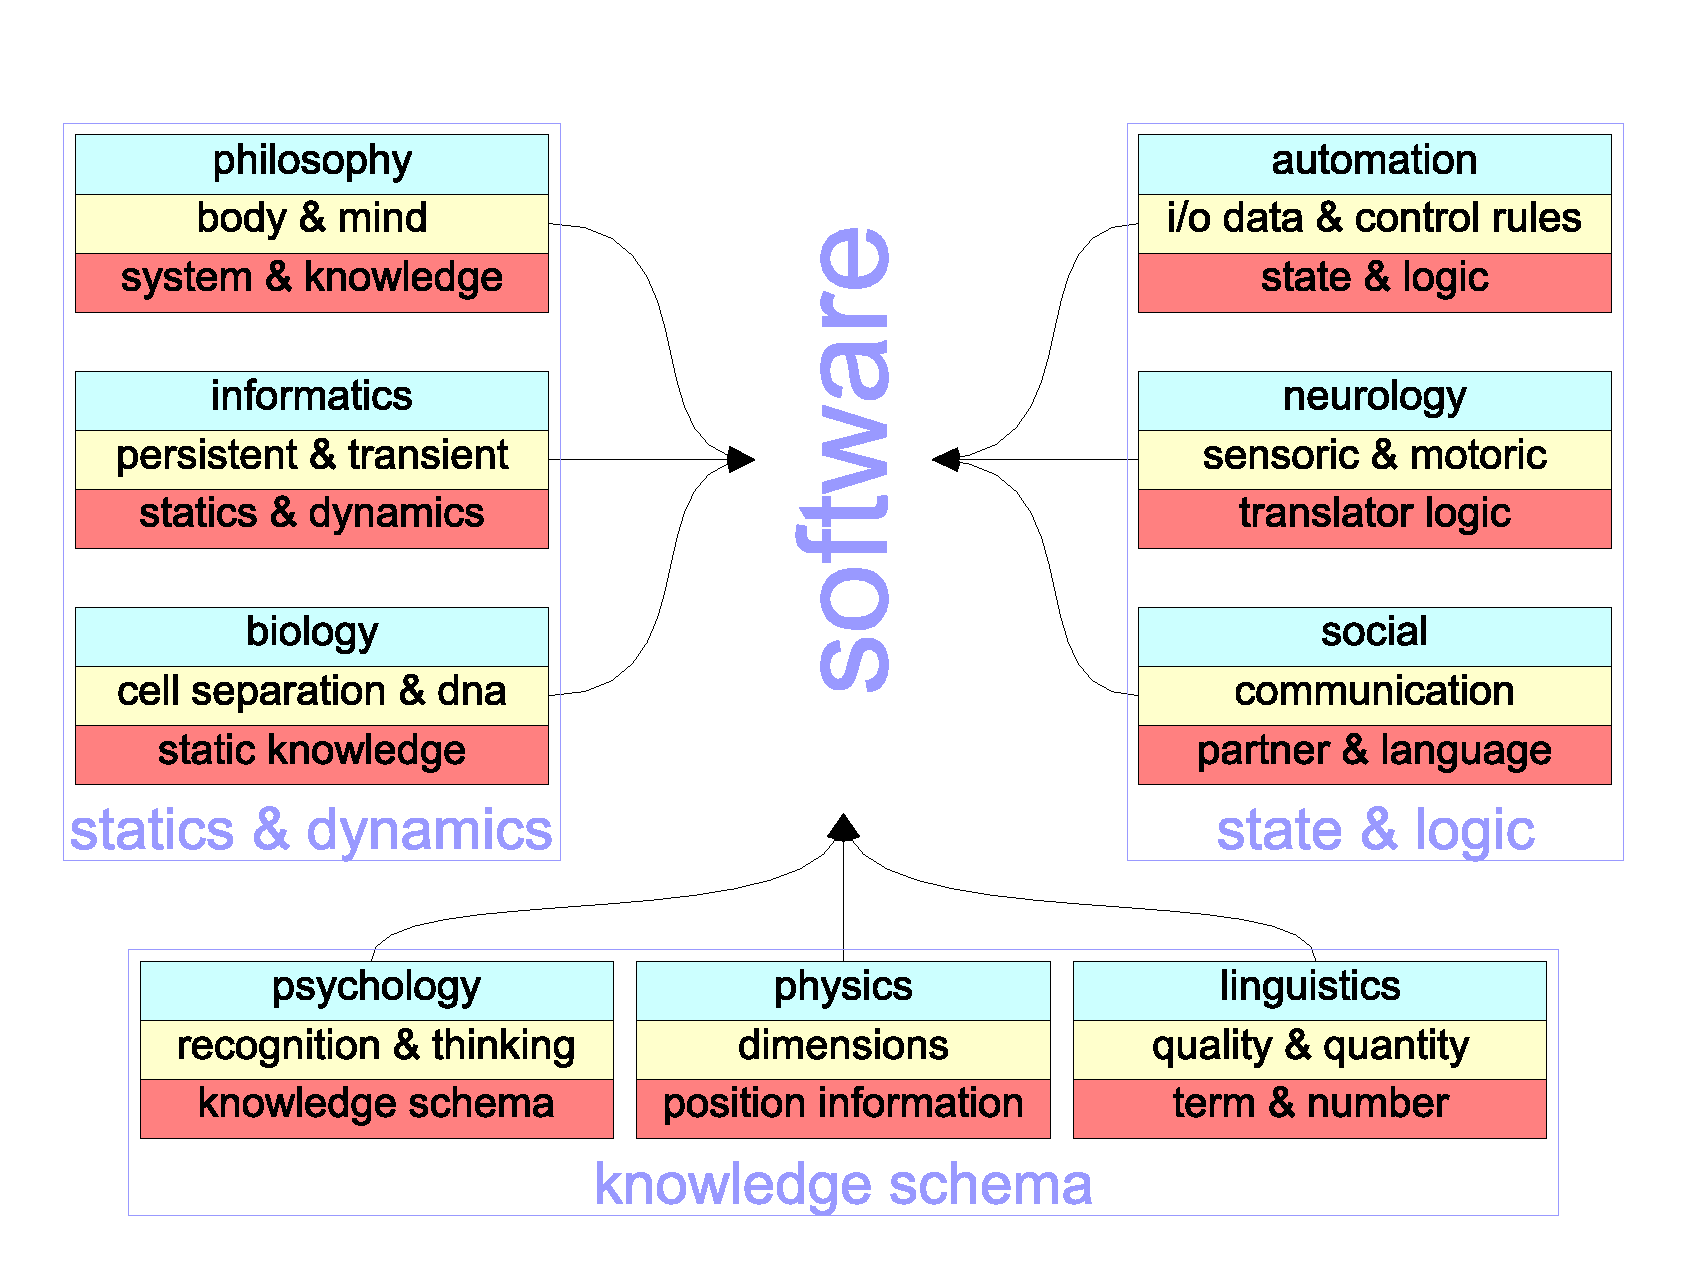
\includegraphics[scale=0.2]{vector/mindmap.eps}
        \caption{Mindmap of Influential Sciences}
        \label{mindmap_figure}
    \end{center}
\end{figure}

Figure \ref{mindmap_figure} shows some of the sciences whose principles were
considered in this work. The name of a field of science is shown on top of each
box. Made observations are mentioned below, in the middle. The resulting design
recommendations for software can be found at the bottom of each box. The
recommendations are grouped into those that justify a separation of
\emph{Statics and Dynamics} (left-hand side), a new kind of
\emph{Knowledge Schema} (lower part of the figure) and a distinction between
\emph{State and Logic} models (right-hand side).

It has to be mentioned though, that only some of the principles underlying a
specific field of science were considered in the figure and in more detail later
in this article. The figure does by no means claim to be complete. The shown
observations are only those that seemed promising in the context of software
design. The existence of persistent and transient data, for example, is only
one of many aspects of the science of informatics. Similarly is the existence
of sensoric and motoric nerve system just one aspect of the field of neurology.
And so on. Further details on the mentioned sciences and observations are not
given here, since later sections will elaborate on some of them.
